\section{Treść zadania}

W labiryncie zbudowanym z kamiennych bloków umieszczono pewną liczbę klejnotów
oraz min.
Niektórych miejscach występują niewielkie wgłębienia.
W labiryncie znajduje się kulisty pojazd, którego zadaniem jest zebranie
wszystkich klejnotów w najmniejszej liczbie ruchów.
Pojazd może poruszać się w dowolnym z 8 kierunków.
Jeżeli pojazd rozpocznie ruch w danym kierunku to zatrzymuje się dopiero
albo we wgłębieniu albo na kamiennym bloku.
Pojazd nie może wtoczyć się na minę.

Na wejściu podana jest zawartość planszy oraz maksymalna liczba ruchów jakich
należy szukać.

\section{Interpretacja wejścia}

Na podstawie wejścia budowany jest graf możliwych ruchów.
Każdy wierzchołek odzwierciedla poprawną\footnote{poprawną, czyli taką
w której pojazd w rzeczywistości może się zatrzymać, zgodnie z regułami gry}
pozycję pojazdu na planszy.
Z każdą krawędzią powiązany jest zbiór diamentów, które można zebrać wykonując
dany ruch.

Oczywiście w grafie nie znajdują się ruchy, które spowodują wejście na minę.

\subsection*{Przykład}

Poniższe wejście (listing~\ref{fig:example1-code}) wygeneruje graf
z rysunku~\ref{fig:example1-graph}.
Pozycje na planszy są oznaczone jako pary, liczone od zera.
Pozycje diamentów znajdują się na krawędziach.

\vspace{1cm}

\begin{minipage}{0.5\textwidth}
    \centering
    \begin{lstlisting}[gobble=8,xleftmargin=.4\textwidth]
        5 6
        20
        ######
        # #+*#
        #+#* #
        #. O+#
        ######
    \end{lstlisting}
    \captionof{lstlisting}{Przykładowe wejście}\label{fig:example1-code}
\end{minipage}
~
\begin{minipage}{0.5\textwidth}
    \centering
    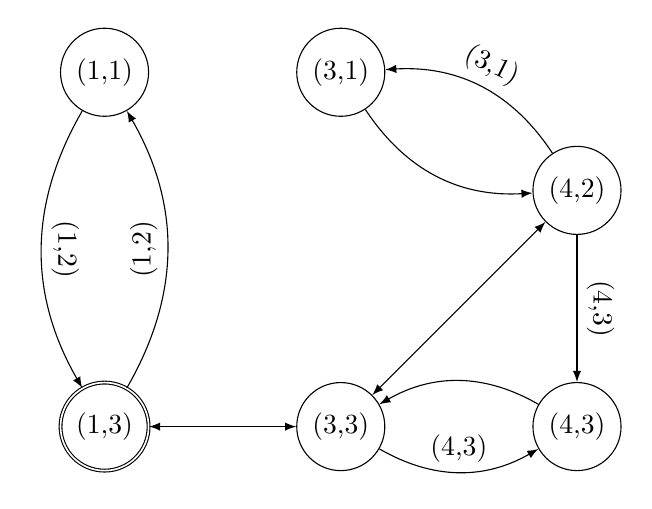
\begin{tikzpicture}[x=3cm,y=-1.5cm]
    \node[draw, circle] (11) at (1,1) {(1,1)};
    \node[draw, circle] (31) at (2,1) {(3,1)};
    \node[draw, circle] (42) at (3,2) {(4,2)};
    \node[draw, circle, double] (13) at (1,4) {(1,3)};
    \node[draw, circle] (33) at (2,4) {(3,3)};
    \node[draw, circle] (43) at (3,4) {(4,3)};

    \draw[->, >=latex] (11) edge [bend right]
    node [midway, above, sloped] {(1,2)} (13);

    \draw[->, >=latex] (31) edge [bend right] (42);

    \draw[->, >=latex] (42) edge
    node [midway, above, sloped] {(4,3)} (43);
    \draw[->, >=latex] (42) edge [bend right]
    node [midway, above, sloped] {(3,1)} (31);

    \draw[->, >=latex] (13) edge [bend right]
    node [midway, above, sloped] {(1,2)} (11);

    \draw[->, >=latex] (33) edge [bend right]
    node [midway, above, sloped] {(4,3)} (43);

    \draw[->, >=latex] (43) edge [bend right] (33);

    \draw[<->, >=latex] (33) edge (42);
    \draw[<->, >=latex] (33) edge (13);
\end{tikzpicture}


    \captionof{figure}{Wygenerowany graf}\label{fig:example1-graph}
\end{minipage}

\section{Strategia szukania rozwiązań}

Aby znaleźć rozwiązanie należy przeszukiwać graf za pomocą algorytmu BFS.
Użycie algorytmu DFS byłoby bardzo nieefektywne w przypadku gdy istnieje
rozwiązanie mające dużo mniej ruchów niż podane maksimum.
Dodatkowo generowane grafy przeważnie mają bardzo dużo cykli więc
DFS zmuszałby do trawersowania grafu po ścieżkach bardzo nieoptymalnych.
Sytuacja ta zilustrowana jest na rysunku~\ref{fig:dfs-vs-bfs}.

W przypadku użycia DFS, po przejściu przez B do C (czerwona ścieżka) jesteśmy
zmuszeni przeglądnąć całą resztę grafu.
Gdy użyjemy BFS, będąc w C (ścieżka czerwona) jesteśmy w stanie stwierdzić,
że już tu byliśmy i wtedy mieliśmy lepszy stan\footnotemark{} (niebieska ścieżka).
Wtedy można zaprzestać dalszego przeszukiwania.

\footnotetext{lepszy stan --- np.\@ tyle samo zebranych diamentów, lecz krótsza ścieżka}

\vspace{1cm}

\begin{figure}[!h]
    \centering
    \begin{subfigure}[b]{0.4\textwidth}
        \centering
        \input{document/tikz/dfs-vs-bfs-dfs.tikz}
        \caption{DFS}
    \end{subfigure}
    \begin{subfigure}[b]{0.4\textwidth}
        \centering
        \begin{tikzpicture}[x=1.8cm,y=-1.8cm,minimum size=1cm]
    \node[draw, circle, double] (a) at (2,0) {A};
    \node[draw, circle] (b) at (1,1) {B};
    \node[draw, circle] (c) at (3,1) {C};

    \node[draw, cloud, cloud puffs=9] (e) at (3.5,0) {graph};

    \draw[->, >=latex, red] (a) -- (b);
    \draw[->, >=latex] (b)
    edge [decoration={snake,post length=5pt}, decorate, red]
    node [below] {long path} (c);

    \draw[->, >=latex, blue] (a) -- (c);
    \draw[->, >=latex, blue] (c) -- (e);
\end{tikzpicture}

        \caption{BFS}
    \end{subfigure}
    \caption{Przykład możliwości zapobiegania wybieraniu nieoptymalnych ścieżek}
    \label{fig:dfs-vs-bfs}
\end{figure}




\begin{algorithm}
    \caption{Pseudokod algorytmu szukającego rozwiązania w grafie}\label{algo:bfs}
    \begin{algorithmic}[1]
        \Procedure{BFS\_diaminy}{}
        \State queue <- empty queue
        \State computed <- array indexed by positions
        \item[]
        \State queue.push(initial\_state)
        \item[]
        \For {pos <- all positions}
        \State computed[pos] <- empty list
        \EndFor
        \item[]

        \While {not queue.empty()}
        \State current <- queue.pop()
        \item[]

        \If {current has all diamonds}
        \State \textbf{return} current.moves
        \EndIf
        \item[]

        \If {current.moves.size() >= max moves}
        \State \textbf{continue}
        \EndIf
        \item[]

        \If {computed[current.position] has a better state}
        \State \textbf{continue}
        \EndIf
        \item[]

        \State computed[current.position].add(current)
        \item[]

        \For {child <- adjacent[current.position]}
        \State queue.push(child)
        \EndFor
        \EndWhile
        \item[]

        \State \textbf{return} no solution
        \EndProcedure
    \end{algorithmic}
\end{algorithm}
